\chapter{Specific Requirements}

\section{External interface Requirements}
\subsection{User Interfaces}
The images below will present an idea of the user interfaces of the major function of the system. Since educators and students uses the platform differently, they will have access to two different personalized dashboard. \newline
Button are coloured in yellow and represents the main function that the CKB platform offers. The green fields instead represent area where the user must enter information (forms-like). \newline

The figure \ref{fig:login-signin} represent the front page to which each user will have access to, and from which he/she can decide to register or log in. 
    
\begin{figure}[H]
    \centering
    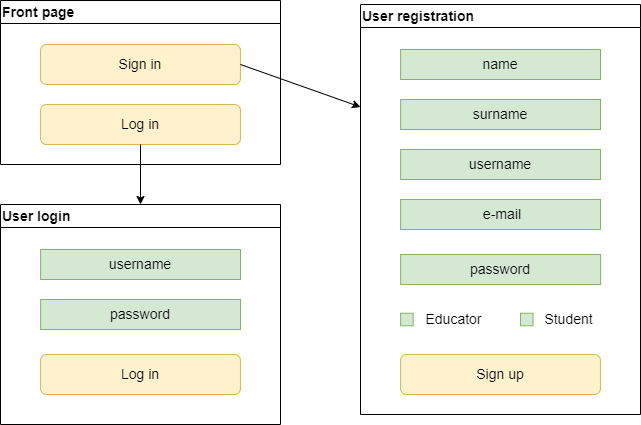
\includegraphics[scale=0.5]{images/login-signin.png}
    \caption{Start page with log in and sign in}
    \label{fig:login-signin}
\end{figure}

\subsubsection{Used by the educators.}
The "All Tournaments" section is the same as the student dashboard in the next image. \newline
The yellow buttons marked with (*) are those that are not always available. For instance in "Manage tournament" the "Close tournament" button is available only when all battles within that tournament are closed. Furthermore, in "Manage battle" the "Perform manual evaluation" button is available only after the final submission deadline of the battle expires and the "Close consolidation stage" button is available only when the educator has performed the manual evaluation.
\begin{figure}[H]
    \centering
    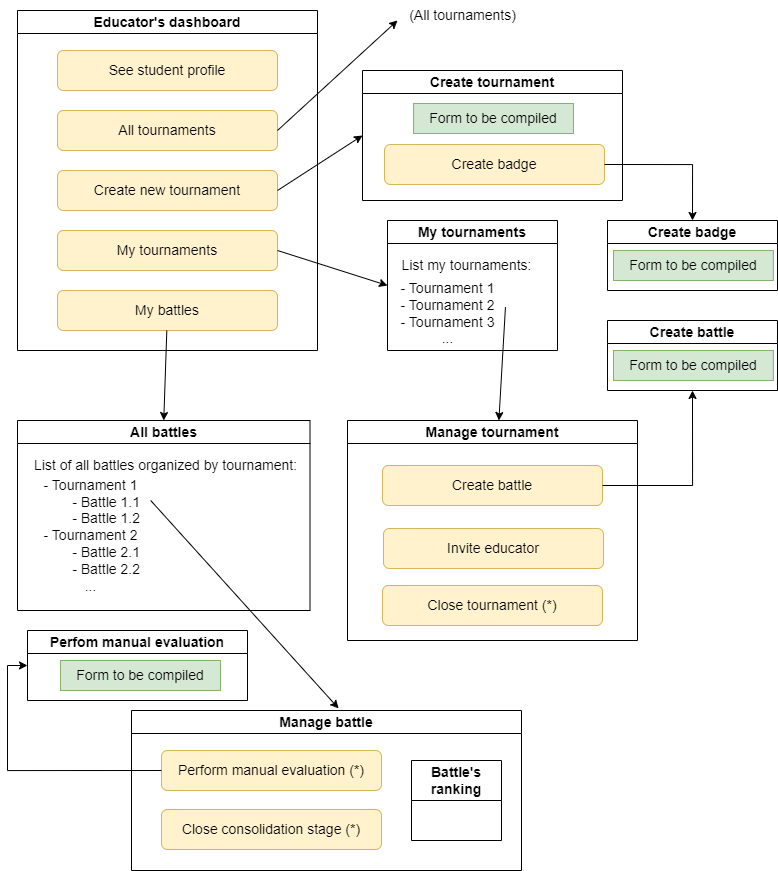
\includegraphics[scale=0.5]{images/educator_dashboard.png}
    \caption{Educator dashboard}
    \label{fig:edDash}
\end{figure}

\subsubsection{Used by the students.}
As stated before yellow buttons marked with (*) are those that are not always available. For instance in "Battle dashboard" both the "Invite student" and "Leave team" buttons are available only when the registration deadline for that battle has not yet expired.
\begin{figure}[H]
    \centering
    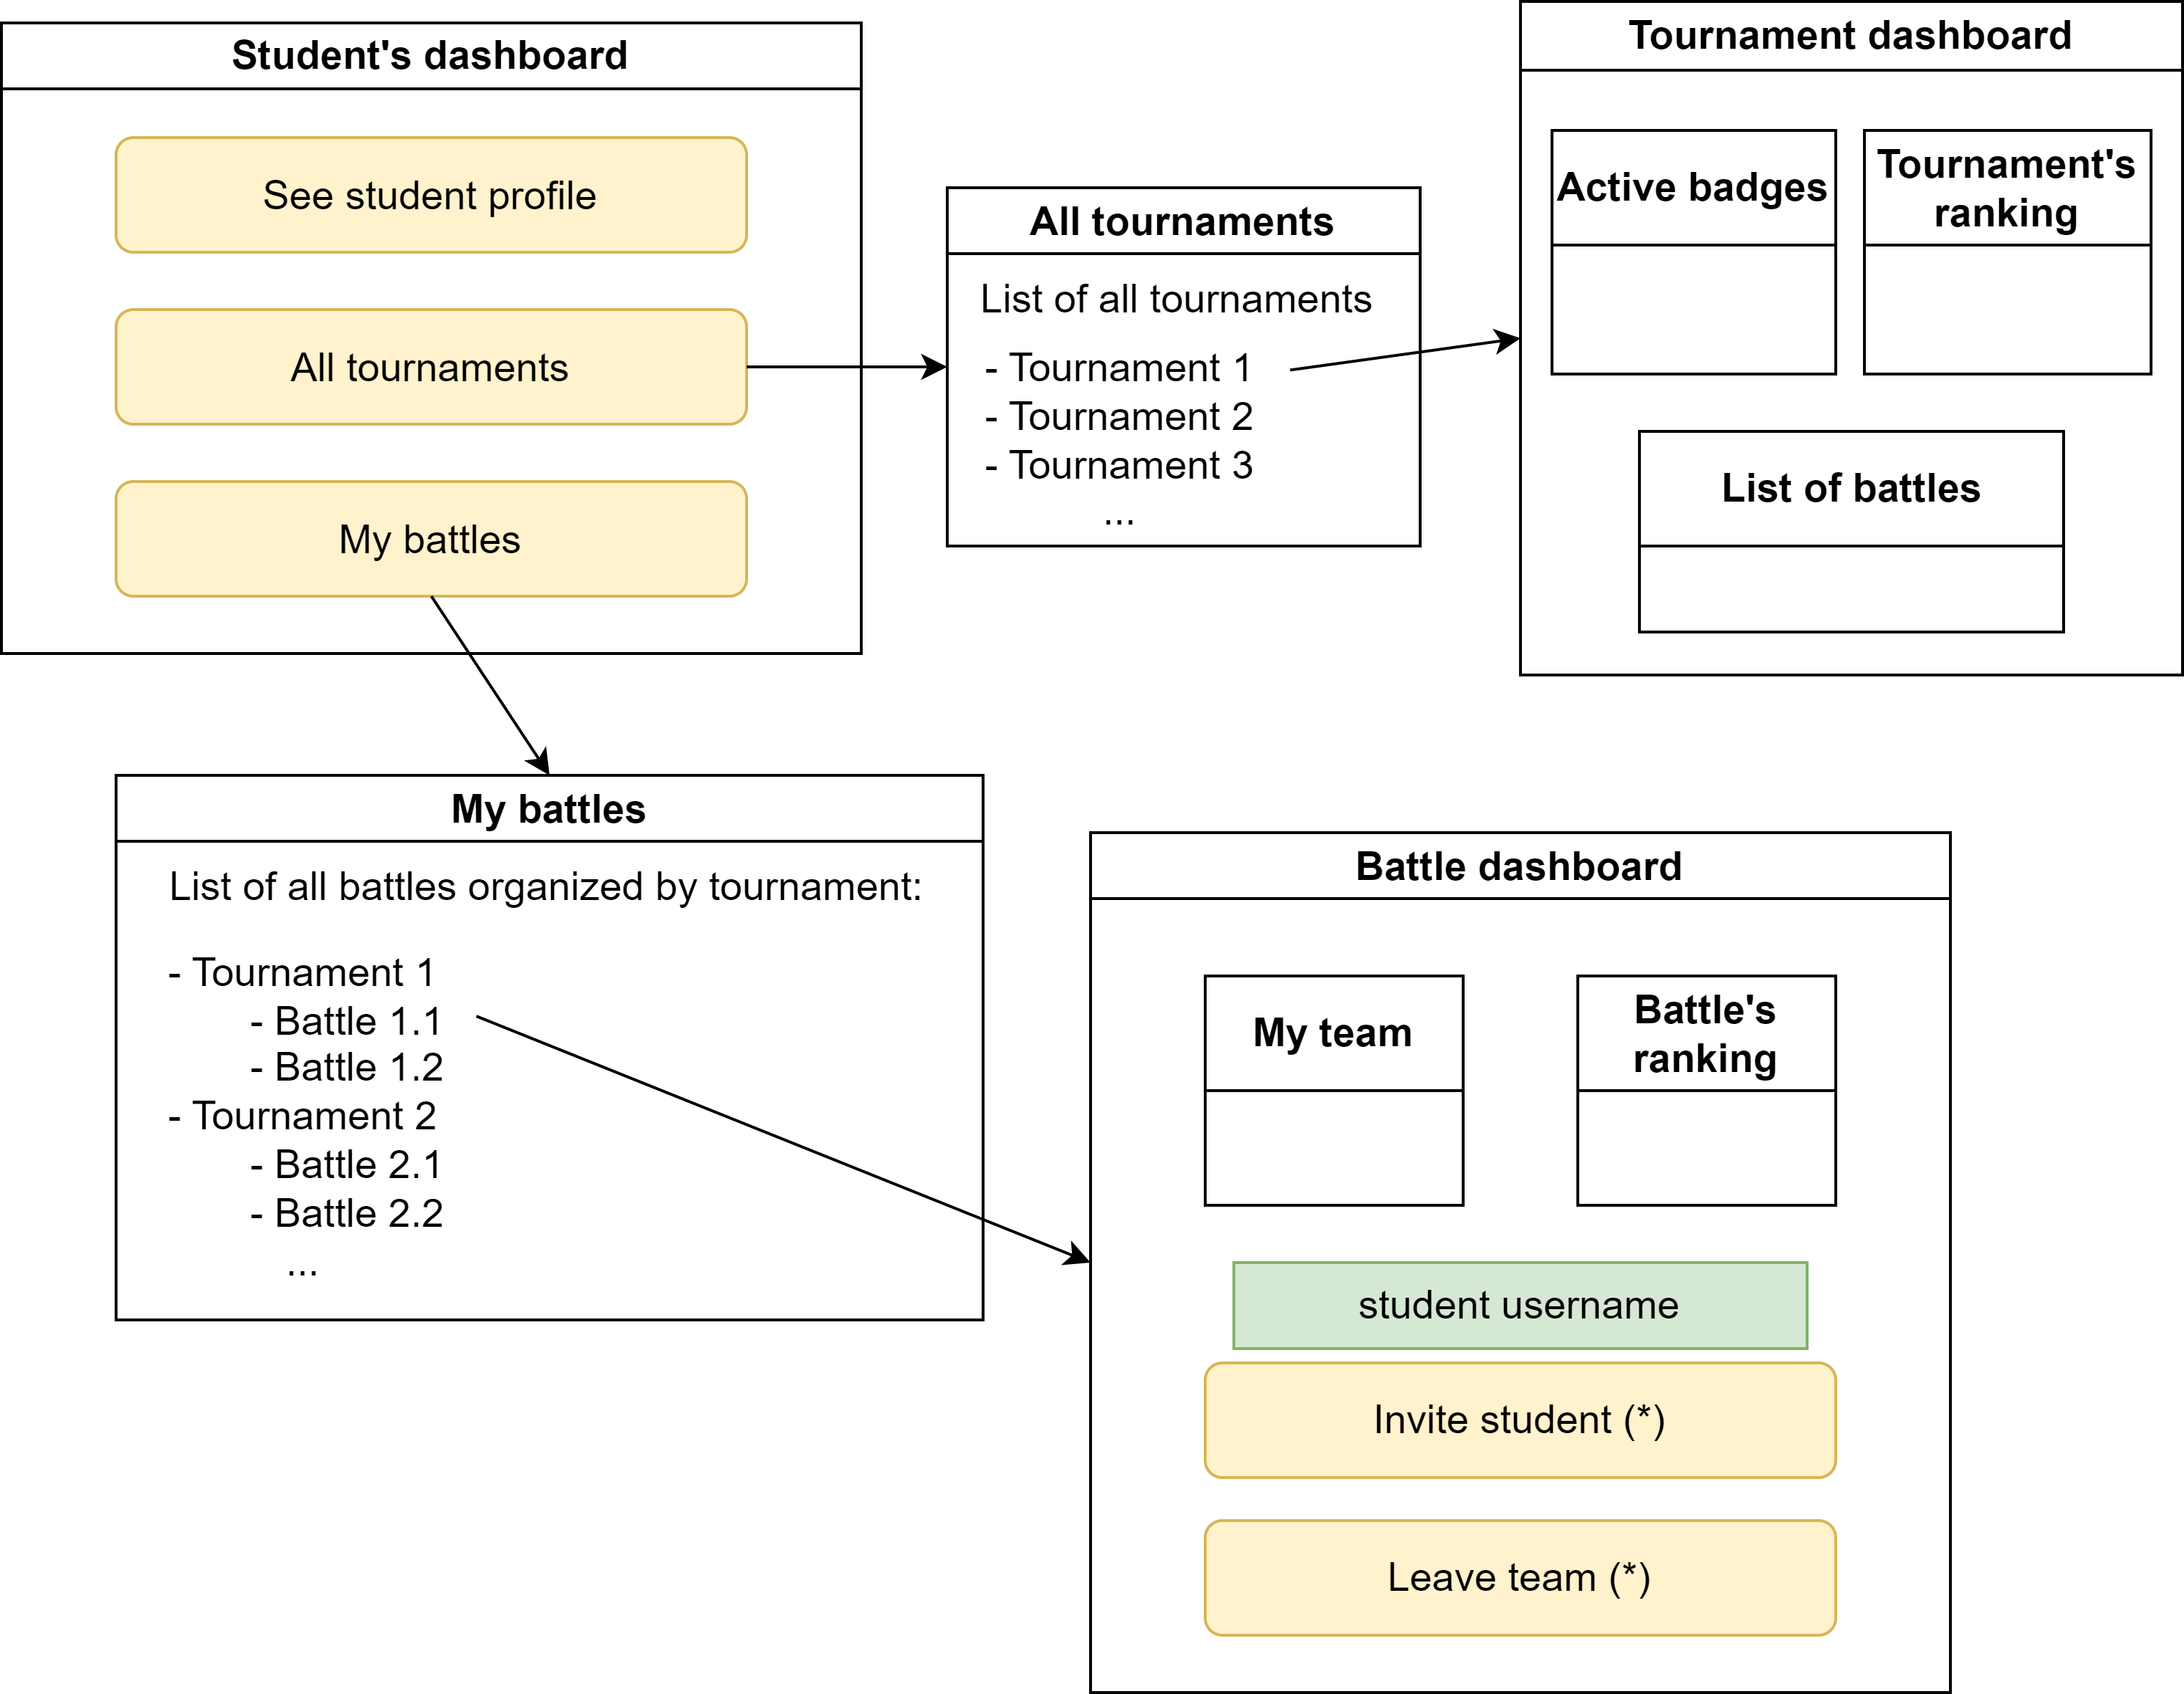
\includegraphics[scale=0.5]{images/student_dashboard.png}
    \caption{Student dashboard}
    \label{fig:stuDash}
\end{figure}

\subsection{Hardware Interfaces}
The only hardware interface required is the personal device of the user (computer, tablet or smartphone) that will access the CKB platform through the web browser.
\subsection{Software Interfaces}
The CKB systems uses the GitHub API in order to automatically detects a new commit to the main branch of each forked repository. This will trigger the automated workflow that will evaluate the current submission.
\subsection{Communication Interfaces}
The only communication interface used is internet, via HTTP.
\clearpage

\section{Functional Requirements}
In this section, it is given a complete description of the functional requirements of the system.

    \subsection{Requirements}
        \begin{enumerate}[label=\textbf{R.\arabic*}]
            \subsubsection*{Users}
            \item \lbl{req: reg} {The system shall allow users to register on the platform with their personal information.}
            \item \lbl{req: login} {The system shall allow registered users to log in the platform with valid credentials.}
            \item \lbl{req: listT} {The system shall allow all users to see the list of ongoing tournaments.}
            \item \lbl{req: evalA} {The system shall automatically evaluate submissions.}
            \item \lbl{req: ranks} {The system shall allow users to be able to monitor ranking in real-time during battles and tournaments.}
            \item \lbl{req: profile} {The system shall allow users to see other students' profile.}
            
            \subsubsection*{Educators}
            \item \lbl{req: createT} {The system shall allow the educators to create tournaments.}
            \item \lbl{req: manageT} {The system shall allow the educators to manage their tournaments, in particular invites other collaborators and ends the tournament.}
            \item \lbl{req: createB} {The system shall allow the educators to create code kata battles within a tournament.}
             \item \lbl{req: evalM} {The system shall allow educators to manually evaluate students (if needed) right after a battle closes, during the consolidation stage.}
            \item \lbl{req: createBad} {The system shall allow educators to create badges.}
            \item \lbl{req: defineRV} {The system shall allow educators to define rules and variables.}

            \subsubsection*{Students}
            \item \lbl{req: enrollT} {The system shall allow students to subscribe in tournaments.}
            \item \lbl{req: enrollB} {The system shall allow students to enroll in a battle within a tournament.}
            \item \lbl{req: formTeam} {The system shall allow students to form team for battles, by inviting other students.}        
            \item \lbl{req: notifT} {The system shall notify the students about new tournaments within 10 seconds.}
            \item \lbl{req: notifB} {The system shall notify the students about upcoming battles in tournaments in which they are subscribed within 10 seconds.}
             \item \lbl{req: notifInvite} {The system shall notify the students when they receive an invite to participate in a team within 10 seconds.}
             \item \lbl{req: notifGitHub} {The system shall notify the students when the GitHub repository of a battle is available.}
             \item \lbl{req: notifRankB} {The system shall notify the students when the final battle rank became available within 10 seconds.}
             \item \lbl{req: notifRankT} {The system shall notify the students when the final tournament rank became available within 10 seconds.}
        \end{enumerate}

    \subsection{Goal mapping on requirements and domain assumption}      
        \begin{center}
            \begin{tabular}{ |m{13.5cm}| }
                \hline \\
                \textbf{\print{goal: manageT}} \\
                \hline \\
                \print{req: reg}
                \print{req: login}
                \print{req: createT} 
                \print{req: manageT}
                \print{req: notifT} \\ 
                \hline \\
                \print{da: internet} 
                \print{da: eduQual} \\
                \hline
            \end{tabular} 
        \end{center}
        \begin{center}   
             \begin{tabular}{|m{13.5cm}|}
                \hline \\
                \textbf{\print{goal: createB}} \\
                \hline \\
                \print{req: reg}
                \print{req: login}
                \print{req: createB} 
                \print{req: notifB}\\
                \hline \\
                \print{da: internet} 
                \print{da: correctCode} 
                \print{da: eduQual} \\
                \hline
            \end{tabular} 
        \end{center} 
        \begin{center}
            \begin{tabular}{|m{13.5cm}|}
                \hline \\
                \textbf{\print{goal: enrollT}} \\
                \hline \\
                \print{req: reg}
                \print{req: login}
                \print{req: listT}
                \print{req: enrollT} 
                \print{req: notifT} \\
                \hline \\
                \print{da: internet}\\
                \hline
            \end{tabular} 
        \end{center}
        \begin{center}
            \begin{tabular}{|m{13.5cm}|}
                \hline \\
                \textbf{\print{goal: enrollB}} \\
                \hline \\
                \print{req: reg}
                \print{req: login}
                \print{req: enrollB} 
                \print{req: notifB} 
                \print{req: notifGitHub} \\
                \hline \\
                \print{da: internet} 
                \print{da: GitHubAccount}
                \print{da: devEnv}\\
                \hline
            \end{tabular} 
        \end{center}
        \begin{center}
            \begin{tabular}{|m{13.5cm}|}
                \hline \\
                \textbf{\print{goal: formTeam}} \\
                \hline \\
                \print{req: reg}
                \print{req: login}
                \print{req: formTeam} 
                \print{req: notifInvite} \\
                \hline \\
                \print{da: GitHubAccount}
                \print{da: devEnv}
                \print{da: GitHubFork}
                \print{da: internet} \\
                \hline
            \end{tabular} 
        \end{center}
        \begin{center}
            \begin{tabular}{|m{13.5cm}|}
                \hline \\
                \textbf{\print{goal: scoreB}} \\
                \hline \\
                \print{req: reg}
                \print{req: login}
                \print{req: evalA} 
                \print{req: evalM} 
                \print{req: ranks} 
                \print{req: notifRankB} \\
                \hline \\
                \print{da: internet} 
                \print{da: autWorkFlow}\\
                \hline
            \end{tabular} 
        \end{center}
        \begin{center}
            \begin{tabular}{|m{13.5cm}|}
                \hline \\
                \textbf{\print{goal: listT}} \\
                \hline \\
                \print{req: reg}
                \print{req: login}
                \print{req: listT} 
                \print{req: notifT}\\
                \hline \\
                \print{da: internet} \\
                \hline
            \end{tabular} 
        \end{center}
        \begin{center}
            \begin{tabular}{|m{13.5cm}|}
                \hline \\
                \textbf{\print{goal: rankT}} \\
                \hline \\
                \print{req: reg}
                \print{req: login}
                \print{req: ranks} 
                \print{req: notifRankT} \\
                \hline \\
                \print{da: internet} \\
                \hline
            \end{tabular} 
        \end{center}
        \begin{center}
            \begin{tabular}{|m{13.5cm}|}
                \hline \\
                \textbf{\print{goal: createBad}} \\
                \hline \\
                \print{req: reg}
                \print{req: login}
                \print{req: createBad}
                \print{req: defineRV}\\
                \hline \\
                \print{da: internet} 
                \print{da: eduQual}
                \print{da: noDuplBadg}\\
                \hline
            \end{tabular} 
        \end{center}
        \begin{center}
            \begin{tabular}{|m{13.5cm}|}
                \hline \\
                \textbf{\print{goal: profile}} \\
                \hline \\
                \print{req: reg}
                \print{req: login}
                \print{req: profile} \\
                \hline \\
                \print{da: internet} \\
                \hline
            \end{tabular} 
        \end{center}
    \clearpage
    
    \subsection{Use cases}
    In figure \ref{fig:use_cases_diagram} is represented a general overview of all use cases deduced from the scenarios in section \ref{desc:scenarios}. All cases include "User login" because all function provided by the platform are accessible to registered users. (except for use registration)
    \begin{figure}[H]
        \centering
        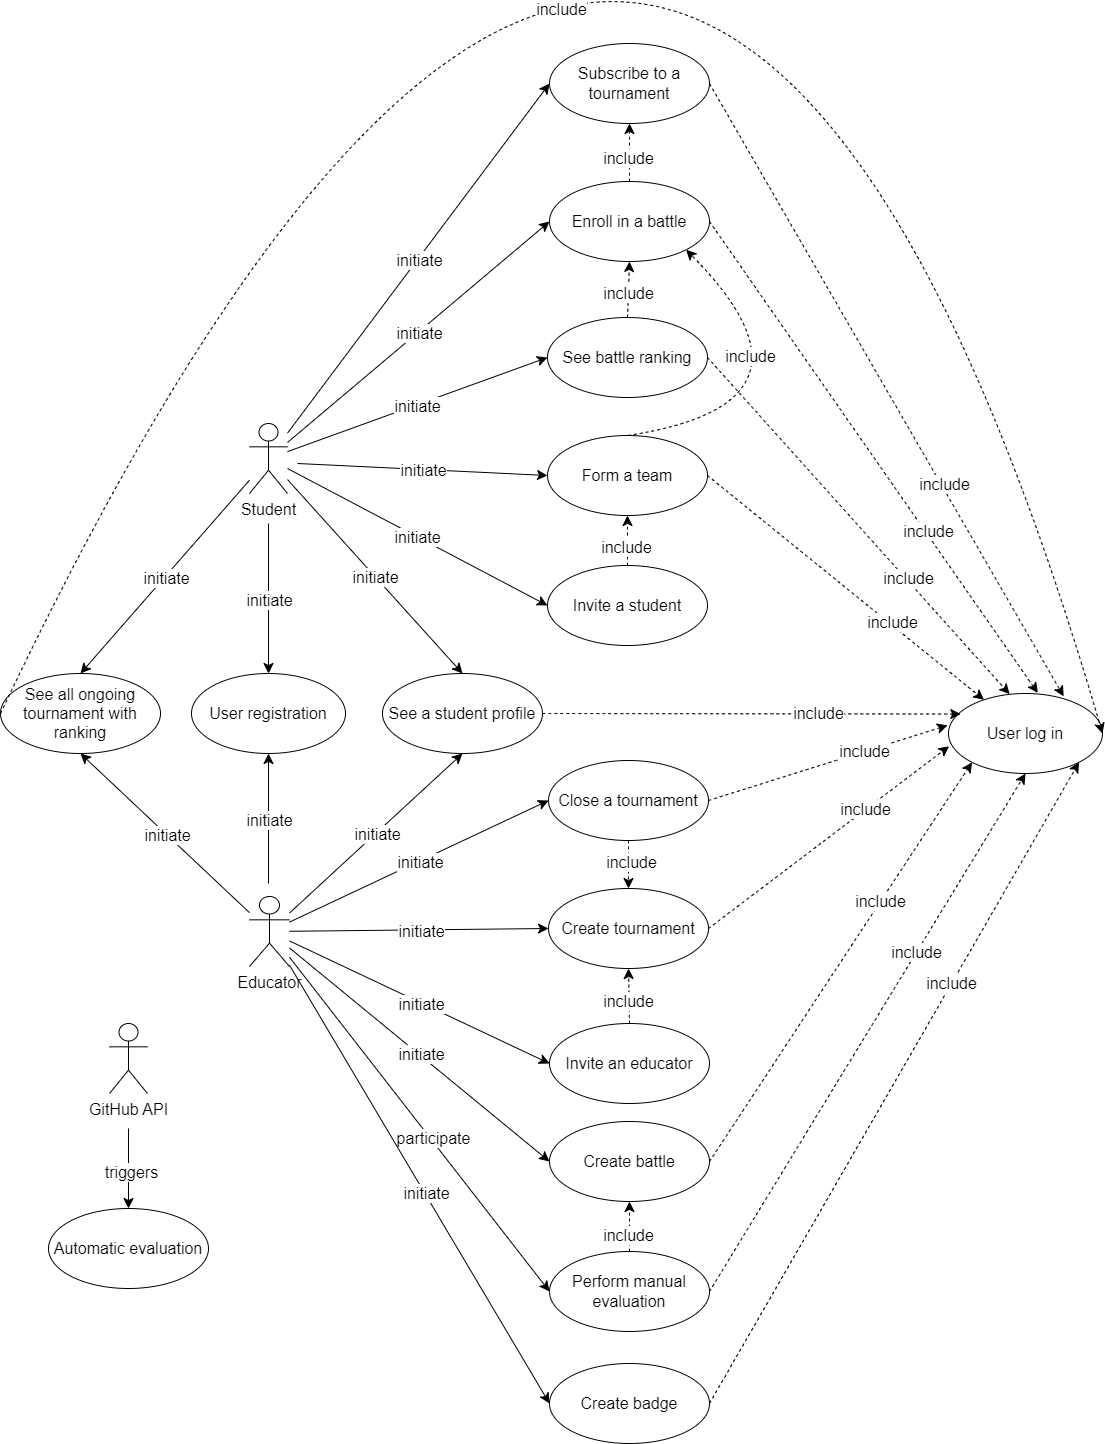
\includegraphics[scale=0.35]{images/use_cases_diagram.png}
        \caption{Use cases diagram}
        \label{fig:use_cases_diagram}
    \end{figure}
    \clearpage
    
    \begin{enumerate}[label=\textbf{UC.\arabic*}]
        \item \lbl{uc: reg} \textbf{User registration}
        \begin{table}[H]
    	    \centering
                \renewcommand{\arraystretch}{1.5}
                \begin{tabular}{|m{3.2cm}|m{9.8cm}|}
                    \hline
                    \textbf{Name} & User registration. \\
                    \hline
                    \textbf{Actors} & Educators, Students. \\
                    \hline
                    \textbf{Entry conditions}  & An user enters the CKB platform for the first time. \\
                    \hline
                    \textbf{Event flow}  & 
                    \begin{enumerate}[label=\arabic*.]
                        \item The user visualize the register page.
                        \item The user inserts the requested personal information.
                        \item The user clicks on the "sign up" button.
                        \item The system checks if the username is available.
                        \item The system sends a confirmation e-mail to the user.
                        \item The user clicks on the link on the confirmation e-mail received.
                        \item The system creates the personal profile of the user.
                    \end{enumerate}\\
                    \hline
                    \textbf{Exit conditions}  & The user is registered in the system. \\
                    \hline
                    \textbf{Exceptions}  & 
                    \begin{itemize}
                        \item If the chosen username is not available the system will throw an error message and the user will be requested to choose another one.
                    \end{itemize} \\
                    \hline 
                \end{tabular}
        \end{table}
        \item \lbl{uc: login} \textbf{User login}
        \begin{table}[H]
    	    \centering
                \renewcommand{\arraystretch}{1.5}
                \begin{tabular}{|m{3.2cm}|m{9.8cm}|}
                    \hline
                    \textbf{Name} & User login.\\
                    \hline
                    \textbf{Actors} &  Educators, students. \\
                    \hline
                    \textbf{Entry conditions}  & The user opens the CKB platform and clicks on "log in" button. \\
                    \hline
                    \textbf{Event flow}  & 
                    \begin{enumerate}[label=\arabic*.]
                        \item The user visualize the log in page.
                        \item The user inserts username and password in the form.
                        \item The user clicks on "log in" button.
                        \item The system checks the credentials.
                        \item The system show the personal dashboard.
                    \end{enumerate}\\
                    \hline
                    \textbf{Exit conditions}  & The user has entered the CKB platform successfully. \\
                    \hline
                    \textbf{Exceptions}  & If username and/or password are not correct the system will throw an error message and return to the entry condition. \\
                    \hline 
                \end{tabular}
        \end{table}
        \item \lbl{uc: createT} \textbf{Create a tournament}
        \begin{table}[H]
    	    \centering
                \renewcommand{\arraystretch}{1.5}
                \begin{tabular}{|m{3.2cm}|m{9.8cm}|}
                    \hline
                    \textbf{Name} & Create a tournament. \\
                    \hline
                    \textbf{Actors} & Educators. \\
                    \hline
                    \textbf{Entry conditions}  & An educator, who is logged in the platform, clicks on the button "create tournament". \\
                    \hline
                    \textbf{Event flow}  &  
                    \begin{enumerate}[label=\arabic*.]
                        \item The educator inserts all needed information in the form.
                        \item The system checks that the correctness of all information.
                    \end{enumerate}\\
                    \hline
                    \textbf{Exit conditions}  & The tournament has been successfully created and can be visualize in the list of all ongoing tournaments. All registered students will receive a notification that a new tournament is available.\\
                    \hline
                    \textbf{Exceptions}  & 
                    If there are some incorrect information, the system will throw an error message and the educator will be requested to modify it. The system return to the entry condition. \\
                    \hline 
                \end{tabular}
        \end{table}
        \item \lbl{uc: createB} \textbf{Create battle}
        \begin{table}[H]
    	    \centering
                \renewcommand{\arraystretch}{1.5}
                \begin{tabular}{|m{3.2cm}|m{9.8cm}|}
                    \hline
                    \textbf{Name} & Create a battle. \\
                    \hline
                    \textbf{Actors} & Educators. \\
                    \hline
                    \textbf{Entry conditions}  &  An educator, who is logged in the platform, wants to create a battle.\\
                    \hline
                    \textbf{Event flow}  & 
                    \begin{enumerate}[label=\arabic*.]
                        \item The educator clicks on the button "my tournaments".
                        \item The educator visualize a list of tournaments to which he/she has access.
                        \item The educator select a tournament from the list.
                        \item The educator clicks on the button "create battle".
                        \item The educator inserts all needed information in the form.
                        \item The system checks that the correctness of all information.
                    \end{enumerate}\\
                    \hline
                    \textbf{Exit conditions}  & The battle has been successfully created and all students subscribed to the tournament in which it belongs have received a notification.  \\
                    \hline
                    \textbf{Exceptions}  &  If there are some incorrect information, the system will throw an error message and the educator will be requested to modify it.  The system return to the entry condition. \\
                    \hline 
                \end{tabular}
        \end{table}
        \item \lbl{uc: inviteE} \textbf{Invite an educator}
        \begin{table}[H]
    	    \centering
                \renewcommand{\arraystretch}{1.5}
                \begin{tabular}{|m{3.2cm}|m{9.8cm}|}
                    \hline
                    \textbf{Name} & Invite an educator. \\
                    \hline
                    \textbf{Actors} & Educators. \\
                    \hline
                    \textbf{Entry conditions}  & An educator, who created a tournament, wants to invite some colleagues to participate. \\
                    \hline
                    \textbf{Event flow}  & 
                    \begin{enumerate}[label=\arabic*.]
                        \item The educator clicks on the button "my tournaments".
                        \item The educator visualize a list of tournaments to which he/she has access.
                        \item The educator select a tournament from the list.
                        \item The educator clicks on the button "invite educator"
                        \item The educator insert the username of the colleague he/she wants to invite.
                        \item The system sends an e-mail to the selected colleague.
                    \end{enumerate}\\
                    \hline
                    \textbf{Exit conditions}  & The invite has been successfully sent. \\
                    \hline
                    \textbf{Exceptions} & If the selected username does not exist or belongs to a student the system will throw an error message. The system will return to the entry conditions.
                \end{tabular}
        \end{table}
        \item \lbl{uc: closeT} \textbf{Close a tournament}
        \begin{table}[H]
    	    \centering
                \renewcommand{\arraystretch}{1.5}
                \begin{tabular}{|m{3.2cm}|m{9.8cm}|}
                    \hline
                    \textbf{Name} & Close a tournament. \\
                    \hline
                    \textbf{Actors} & Educators. \\
                    \hline
                    \textbf{Entry conditions}  &  An educator, who created a tournament, wants close it. \\
                    \hline
                    \textbf{Event flow}  & 
                    \begin{enumerate}[label=\arabic*.]
                        \item The educator clicks on the button "my tournaments"
                        \item The educator visualize a list of tournaments to which he/she has access.
                        \item The educator select a tournament from the list.
                        \item The educator clicks on the button "close tournament".
                        \item The system checks whether all battles in that tournament are finished.
                    \end{enumerate}\\
                    \hline
                    \textbf{Exit conditions}  & The tournament has been successfully closed. \\
                    \hline
                    \textbf{Exceptions}  & If not all battles of the tournament are over, the system will throw an error message and the educator will not be able to close the tournament. The system returns to the entry condition.\\
                    \hline 
                \end{tabular}
        \end{table}
        \item \lbl{uc: rankT} \textbf{Visualize all ongoing tournament with ranking}
        \begin{table}[H]
    	    \centering
                \renewcommand{\arraystretch}{1.5}
                \begin{tabular}{|m{3.2cm}|m{9.8cm}|}
                    \hline
                    \textbf{Name} & Visualize all ongoing tournament with ranking.  \\
                    \hline
                    \textbf{Actors} & Educators and students. \\
                    \hline
                    \textbf{Entry conditions}  & A user wants to see the list of all tournaments and/or their rankings. \\
                    \hline
                    \textbf{Event flow}  & 
                    \begin{enumerate}[label=\arabic*.]
                        \item The user clicks on the button "see all tournaments"
                        \item The user visualize a list of tournaments.
                        \item The user clicks on a tournament to visualize its ranking.
                    \end{enumerate}\\
                    \hline
                    \textbf{Exit conditions}  & The user visualize a list of tournaments and/or a specific ranking. \\
                    \hline
                \end{tabular}
        \end{table}
        \item \lbl{uc: enrollT} \textbf{Subscribe to a tournament}
        \begin{table}[H]
    	    \centering
                \renewcommand{\arraystretch}{1.5}
                \begin{tabular}{|m{3.2cm}|m{9.8cm}|}
                    \hline
                    \textbf{Name} & Subscribe to a tournament.\\
                    \hline
                    \textbf{Actors} & Students. \\
                    \hline
                    \textbf{Entry conditions}  & A student, who is registered to the platform, receive a notification that a new tournament is available and wants to subscribe.\\
                    \hline
                    \textbf{Event flow}  & 
                    \begin{enumerate}[label=\arabic*.]
                        \item The user clicks on the link received via e-mail.
                        \item The system check if the subscription deadline is not expired.
                    \end{enumerate}\\ 
                    \hline
                    \textbf{Exit conditions}  & The student is successfully subscribed to the tournament. The system will send the student further notification about the upcoming battles. \\
                    \hline
                    \textbf{Exceptions}  & If the subscription deadline is expired, the system will throw an error message and the student will not be able to subscribe to the tournament. The system will return to the entry condition. \\
                    \hline 
                \end{tabular}
        \end{table}
        \item \lbl{uc: enrollB} \textbf{Enroll in a battle}
        \begin{table}[H]
    	    \centering
                \renewcommand{\arraystretch}{1.5}
                \begin{tabular}{|m{3.2cm}|m{9.8cm}|}
                    \hline
                    \textbf{Name} & Enroll in a battle. \\
                    \hline
                    \textbf{Actors} & Students. \\
                    \hline
                    \textbf{Entry conditions}  & A student, who is subscribed to a tournament, receive a notification that a new battle is available and wants to enroll.\\
                    \hline
                    \textbf{Event flow}  & 
                    \begin{enumerate}[label=\arabic*.]
                        \item The student clicks on the link received by e-mail.
                        \item The system checks if the registration deadline is not expired.
                    \end{enumerate}\\ 
                    \hline
                    \textbf{Exit conditions}  & The student is successfully enrolled to the battle. \\
                    \hline
                    \textbf{Exceptions}  & If the registration deadline is expired, the system will throw an error message and the student will not be able to subscribe to the battle. The system will return to the list of battles.  \\
                    \hline 
                \end{tabular}
        \end{table}
        \item \lbl{uc: inviteS} \textbf{Invite a student}
        \begin{table}[H]
    	    \centering
                \renewcommand{\arraystretch}{1.5}
                \begin{tabular}{|m{3.2cm}|m{9.8cm}|}
                    \hline
                    \textbf{Name} & Invite a student. \\
                    \hline
                    \textbf{Actors} & Students. \\
                    \hline
                    \textbf{Entry conditions}  & A student, who is enrolled in a battle, wants to create a team. \\
                    \hline
                    \textbf{Event flow}  &  
                    \begin{enumerate}[label=\arabic*.]
                        \item The student clicks on the button "my battles".
                        \item The student visualizes the list of battles he/she is registered to.
                        \item The student selects a battle.
                        \item The student visualizes his/hers current team.
                        \item The student clicks on the button "invite a student".
                        \item The system checks if the registration deadline is not expired.
                        \item The student inserts the username of the student who he/she wants to invite.
                        \item The system checks if the username inserted is enrolled in the battle.
                    \end{enumerate}\\ 
                    \hline
                    \textbf{Exit conditions}  & The invited student has received an e-mail. \\
                    \hline
                    \textbf{Exceptions}  &
                    \begin{itemize}
                        \item If the registration deadline for the battle is expired, the invite will not be sent.
                        \item If the invited student is not enrolled in the invite will not be sent.
                    \end{itemize} 
                     In both cases the system will throw an error message and return to the entry condition.\\
                    \hline 
                \end{tabular}
        \end{table}
        \item \lbl{uc: leaveT} \textbf{Leave a team}
        \begin{table}[H]
    	    \centering
                \renewcommand{\arraystretch}{1.5}
                \begin{tabular}{|m{3.2cm}|m{9.8cm}|}
                    \hline
                    \textbf{Name} & Leave a team. \\
                    \hline
                    \textbf{Actors} & Students. \\
                    \hline
                    \textbf{Entry conditions}  & A student wants to leave his/hers current team. \\
                    \hline
                    \textbf{Event flow}  & 
                    \begin{enumerate}[label=\arabic*.]
                        \item The student clicks on the button "my battles".
                        \item The student visualizes the list of battles he/she is registered to.
                        \item The student selects a battle.
                        \item The student visualizes his/hers current team.
                         \item The student clicks on the button "leave team".
                        \item The system check if the registration deadline is not expired.
                    \end{enumerate}\\ 
                    \hline
                    \textbf{Exit conditions}  & The student has successfully left his/her team. \\
                    \hline
                    \textbf{Exceptions}  & If the registration deadline is already expired the system will throw an error message and the student will not be able to leave the team. The system will return to the entry condition. \\
                    \hline 
                \end{tabular}
        \end{table}
        \item \lbl{uc: rankB} \textbf{View battle ranking}
        \begin{table}[H]
    	    \centering
                \renewcommand{\arraystretch}{1.5}
                \begin{tabular}{|m{3.2cm}|m{9.8cm}|}
                    \hline
                    \textbf{Name} & View battle ranking. \\
                    \hline
                    \textbf{Actors} & Educators and students. \\
                    \hline
                    \textbf{Entry conditions}  & An user wants to see the real-time ranking of a battle. \\
                    \hline
                    \textbf{Event flow}  & 
                    \begin{enumerate}[label=\arabic*.]
                        \item The user clicks on the button "my battles".
                        \item The user visualizes the list of battles that are correlated to him/her.
                        \item The user selects a battle.
                        \item The system show the real-time raking of the selected battle.
                    \end{enumerate}\\ 
                    \hline
                    \textbf{Exit conditions}  & The user visualize the real-time ranking of a battle. \\
                    \hline
                \end{tabular}
        \end{table}
        \item \lbl{uc: evalM} \textbf{Perform manual evaluation}
        \begin{table}[H]
    	    \centering
                \renewcommand{\arraystretch}{1.5}
                \begin{tabular}{|m{3.2cm}|m{9.8cm}|}
                    \hline
                    \textbf{Name} & Perform manual evaluation. \\
                    \hline
                    \textbf{Actors} & Educators. \\
                    \hline
                    \textbf{Entry conditions}  & An educator wants to manually evaluate some students. \\
                    \hline
                    \textbf{Event flow}  & 
                    \begin{enumerate}[label=\arabic*.]
                        \item The educator clicks on the button "my battles".
                        \item The educator visualize the list of battles that are correlated to him/her.
                        \item The educator select the battle he/she wants to evaluate.
                        \item The educator clicks on the button "perform manual evaluation".
                        \item The educator assigns a personal score to each participant in the battle.
                        \item The educator clicks on the button "end consolidation stage".
                    \end{enumerate}\\ 
                    \hline
                    \textbf{Exit conditions}  &  The educator end the consolidation stage. \\
                    \hline
                \end{tabular}
        \end{table}
        \item \lbl{uc: evalA} \textbf{Perform automatic evaluation}
        \begin{table}[H]
    	    \centering
                \renewcommand{\arraystretch}{1.5}
                \begin{tabular}{|m{3.2cm}|m{9.8cm}|}
                    \hline
                    \textbf{Name} & Perform automatic evaluation. \\
                    \hline
                    \textbf{Actors} & GitHub API. \\
                    \hline
                    \textbf{Entry conditions}  & A team push a new solution on the GitHub repository. \\
                    \hline
                    \textbf{Event flow}  & 
                    \begin{enumerate}[label=\arabic*.]
                        \item The GitHub API triggers the CKB platform.
                        \item The system perform the automatic evaluation.
                        \item The system update the score of each team and the real-time rank.
                    \end{enumerate}\\ 
                    \hline
                    \textbf{Exit conditions}  &  The real-time rank is updated. \\
                    \hline
                \end{tabular}
        \end{table}
        \item \lbl{uc: createBadge} \textbf{Create a badge}
        \begin{table}[H]
    	    \centering
                \renewcommand{\arraystretch}{1.5}
                \begin{tabular}{|m{3.2cm}|m{9.8cm}|}
                    \hline
                    \textbf{Name} & Create a badge. \\
                    \hline
                    \textbf{Actors} & Educators. \\
                    \hline
                    \textbf{Entry conditions}  & An educator wants to create a badge within a tournament. The educator is creating the tournament. \\
                    \hline
                    \textbf{Event flow}  & 
                    \begin{enumerate}[label=\arabic*.]
                        \item The educator clicks on the button "create badge".
                        \item The educator inserts all information requested in a form.
                        \item The system check the correctness of the inserted information.
                    \end{enumerate}\\ 
                    \hline
                    \textbf{Exit conditions}  & The badge has been successfully created. \\
                    \hline
                \end{tabular}
        \end{table}
        \item \lbl{uc: profile} \textbf{See student profile}
        \begin{table}[H]
    	    \centering
                \renewcommand{\arraystretch}{1.5}
                \begin{tabular}{|m{3.2cm}|m{9.8cm}|}
                    \hline
                    \textbf{Name} & See student profile. \\
                    \hline
                    \textbf{Actors} & Educators and students. \\
                    \hline
                    \textbf{Entry conditions}  & An user wants to see a personal profile of a student. \\
                    \hline
                    \textbf{Event flow}  & 
                    \begin{enumerate}[label=\arabic*.]
                        \item The user clicks on the button "see student profile".
                        \item The user inserts the username of the student he/she wants to see.
                        \item The system check the inserted information.
                        \item The system show the personal profile requested if present.
                    \end{enumerate}\\ 
                    \hline
                    \textbf{Exit conditions}  & The user see the personal profile of a student. \\
                    \hline
                    \textbf{Exceptions} & If the selected username does not exist the system will throw an error message. The system will return to the entry conditions \\
                    \hline
                \end{tabular}
        \end{table}
    \end{enumerate}
    

    \subsection{Traceability matrix}
    \begin{table}[h]
	    \centering
            \renewcommand{\arraystretch}{1.5}
            \begin{tabular}{|m{3cm}|m{3cm}|m{3cm}|m{3cm}|}
                \hline
                \textbf{Use Case ID} & \textbf{Goal ID} & \textbf{Req ID} & \textbf{Scenario} \\
                \hline
                \ref{uc: reg} & ALL & \ref{req: reg} & \ref{sce: reg}  \\
                \hline
                \ref{uc: login} & ALL & \ref{req: login} & \ref{sce: reg}   \\
                \hline
                \ref{uc: createT} & \ref{goal: manageT} & \ref{req: createT} & \ref{sce: createTB}   \\
                \null & \null  & \ref{req: manageT}&\null \\
                \null & \null  & \ref{req: notifT}&\null \\
                \hline
                \ref{uc: createB} & \ref{goal: createB} & \ref{req: createB} & \ref{sce: createTB}  \\
                \null & \null  & \ref{req: notifB}&\null \\
                \hline
                \ref{uc: inviteE} & \ref{goal: createB} & \ref{req: manageT} & \ref{sce: createTB}  \\
                \hline
                \ref{uc: closeT} & \ref{goal: manageT} & \ref{req: manageT} & \ref{sce: createTB}  \\
                \hline
                \ref{uc: rankT} & \ref{goal: listT} & \ref{req: listT} & \ref{sce: evalM}  \\
                \null & \null  & \ref{req: notifT}&\null \\
                \null & \ref{goal: rankT}  & \ref{req: ranks}&\null \\
                \null & \null  & \ref{req: notifRankT}&\null \\
                \hline
                \ref{uc: enrollT} & \ref{goal: enrollT} & \ref{req: listT} & \ref{sce: createTB}  \\
                \null & \null  & \ref{req: enrollT}&\null \\
                \null & \null  & \ref{req: notifT}&\null \\
                \hline
                \ref{uc: enrollB} & \ref{goal: enrollB} & \ref{req: enrollB} & \ref{sce: formTeam} \\
                \null & \null  & \ref{req: formTeam}& \null \\ 
                \null & \null  & \ref{req: notifB}&\null \\
                \null & \null  & \ref{req: notifGitHub}&\null \\
                \hline
                \ref{uc: inviteS} & \ref{goal: formTeam} & \ref{req: formTeam} & \ref{sce: formTeam} \\
                \null & \null  & \ref{req: notifInvite}& \null \\ 
                \hline
                \ref{uc: leaveT} & \ref{goal: formTeam} & \ref{req: formTeam} & \ref{sce: formTeam} \\
                \null & \null  & \ref{req: notifInvite}& \null \\ 
                \hline
                \ref{uc: rankB} & \ref{goal: scoreB} & \ref{req: evalA} & \ref{sce: evalA} \\
                \null & \null  & \ref{req: ranks}& \null \\ 
                \null & \null  & \ref{req: evalM}&\null \\
                \null & \null  & \ref{req: notifRankB}&\null \\
                \hline
                \ref{uc: evalM} & \ref{goal: scoreB} & \ref{req: evalM} & \ref{sce: evalM} \\
                \null & \null  & \ref{req: notifRankB}&\null \\
                \hline
                \ref{uc: evalA} & \ref{goal: scoreB} & \ref{req: evalA} & \ref{sce: evalA} \\
                \null & \null  & \ref{req: ranks}&\null \\
                \null & \null  & \ref{req: notifRankB}&\null \\
                \hline

            \end{tabular}
    \end{table}

    \clearpage
    \begin{table}[h]
        \centering
        \renewcommand{\arraystretch}{1.5}
        \begin{tabular}{|m{3cm}|m{3cm}|m{3cm}|m{3cm}|}
            \hline
            \textbf{Use Case ID} & \textbf{Goal ID} & \textbf{Req ID} & \textbf{Scenarios} \\
            \hline
            \ref{uc: createBadge} & \ref{goal: createBad} & \ref{req: createBad} & \ref{sce: badge} \\
            \null & \null  & \ref{req: defineRV}&\null \\
            \hline
            \ref{uc: profile} & \ref{goal: profile} & \ref{req: profile} & \ref{sce: profile} \\
            \hline
        \end{tabular}
    \end{table}
    
\clearpage
\section{Performance Requirements}
In this section are listed some performance requirements for the CKB platform that are essential to the efficiency of the entire system.
The CKB platform should be able to guarantee the connection of 100.000 users simultaneously. \newline 
In less than 2 seconds, it should be able to respond to user interactions, such as page loading. \newline
In less than 5 seconds, it should be able to send a response to a query and run its algorithms on the metadata. This is crucial for having real-time evaluation of the students' submissions.

\section{Design Constraints}
\subsection{Standards Compliance}
The code should follow the requirements contained in this document. Furthermore, its comments should
be clear and focused.
The system will store in the database 3 types of data:
\begin{enumerate}
    \item User main information for example email-Password as primary key, name , surname...
    \item The final rankings of a tournament. The system saves in the database the ranking of a tournament once it's finished.
    \item The final ranking of a battle.
\end{enumerate}

CKB system shall use stateless protocols and standard operations to allow components to
be managed and updated without affecting the system as a whole.
It’s crucial to design modules properly so that ease of use, security and performance will
remain the core factors of the system.
\subsection{Hardware Limitations}
To use CKB the user needs to have a device that's at least can connect to internet and can share code on GitHub.
The device might be connected to internet and to the GitHub account that the user put during the registration. 
\subsection{Other Constraints}
CKB system will send emails to the users and automatically pulls the GitHub main branch of the teams so it's important that the user allows the system to send emails and to join the GitHub project.

\section{Software System Attributes}
\subsection{Reliability}
The CKB platform should be highly reliable in order to guarantee the continuity of the service, every user should be able to access the platform anytime. The system should implements robust errors handling and fault tolerance mechanism to prevent error propagation and data loss. \subsection{Availability}
The CKB platform should be available to users 24/7, without frequent interruptions. 
Since the system is not emergency-related, it should be up 99\% of the time.
This means that the average downtime is around at 3.65 days per year. \newline
In order to achieve this level of availability the system should implement a disaster recovery plan, monitoring and alerting tools, and the ability to react fast to resolve any system issues.
\subsection{Security}
As the system store some personal information about the users, security is an important issue. This stored data must be encrypted, and passwords must also be hashed. \newline
Every time a password need to be recovered a new one must be created, by sending a verification e-mail that contain a time-limited that confirm the user identity and gives them access to reset their password.
\subsection{Maintainability}
The CKB system should be divided in different modules implementing the various functionalities. In this way ordinary maintenance and/or future fixes or improvements will be easier to be performed. \newline
Maintenance and updates must be scheduled in advance so that they do not interfere with ongoing battles. 
\subsection{Portability}
The CKB platform should be accessible from any web browser.
\subsection{Usability}
The user interfaces of the platform should be easy to use and intuitive.

\section{Other Requirements}
\subsection{Privacy Requirements}
At the registration every user is asked to fill the following mandatory fields:
name, surname and e-mail. 
